\documentclass[a4paper,12pt,twoside]{report}

\usepackage{graphicx}
\usepackage[utf8]{inputenc}
\usepackage[T1]{fontenc}
\usepackage{xcolor,graphicx}
\usepackage{ragged2e}
\usepackage[left=2.5cm,right=2.5cm,top=2cm,bottom=3cm]{geometry}

% Created by Yue Li, June 2017

\pagestyle{empty}

\setlength{\parskip}{0em}
\setlength{\parindent}{0em}

\makeatletter  %to avoid error messages generated by "\@". Makes Latex treat "@" like a letter

\linespread{1.5}
\def\submitdate#1{\gdef\@submitdate{#1}}
\def\degree#1{\gdef\@degree{#1}}
\def\studentid#1{\gdef\@studentid{#1}}
\def\supervisor#1{\gdef\@supervisor{#1}}

\def\maketitle{
    
  \begin{titlepage}{
    
    \centering{
    \includegraphics[width=0.5\columnwidth]{images/gmit-logo.png}} \par
    \large{\bf Galway Mayo Institute of Technology} \par
    \normalsize { BACHELOR OF SCIENCE (HONOURS) IN SOFTWARE DEVELOPMENT \par
    Applied Project And Minor Dissertation }
    \vskip 1in \par
    \vskip 1in \par
    \LARGE {\bf \@title}
    
  }
  \vskip 0.3in \par
  \vskip 0.3in \par
  \vskip 0.3in \par
  \vskip 0.3in \par
  \vskip 0.3in \par
  \large {\bf Student Names: \@author} \par
  \large {\bf Student Numbers: \@studentid}
  \vskip 0.3in \par
  \large {\bf Supervised by \@supervisor}

  \end{titlepage}
}

\def\titlepage{
  \newpage
  \centering
  \linespread{1}
  \normalsize
  \vbox to \vsize\bgroup\vbox to 9in\bgroup
}
\def\endtitlepage{
  \par
  \kern 0pt
  \egroup
  \vss
  \egroup
  \cleardoublepage
}

\def\abstract{
  \begin{center}{
    \large\bf Abstract}
  \end{center}
  \small
  %\def\baselinestretch{1.5}
  \linespread{1.5}
  \normalsize
}
\def\endabstract{
  \par
}

\newenvironment{acknowledgements}{
  \cleardoublepage
  \begin{center}{
    \large \bf Acknowledgements}
  \end{center}
  \small
  \linespread{1.5}
  \normalsize
}{\cleardoublepage}
\def\endacknowledgements{
  \par
}

\def\preface{
    \pagenumbering{roman}
    \pagestyle{plain}
    \doublespacing
}

\def\body{
	
    \cleardoublepage    
    \pagestyle{uheadings}
    \tableofcontents
    \pagestyle{plain}
    \cleardoublepage
    \pagestyle{uheadings}
    \listoftables
    \pagestyle{plain}
    \cleardoublepage
    \pagestyle{uheadings}
    \listoffigures
    \pagestyle{plain}
    \cleardoublepage
    \pagestyle{uheadings}
    \pagenumbering{arabic}
    \doublespacing
    
}

\makeatother  %to avoid error messages generated by "\@". Makes Latex treat "@" like a letter

\begin{document}

\title{Final Year Project}
% author names
\author{Your Name}
\submitdate{May 2016}
\degree{BSc Computer Science}
\studentid{Your Student ID}
\supervisor{Your Supervisor Name}

\maketitle

\preface
\section*{Abstract}
\\
Sports and technology are two words which praise one another and have been endeavouring all through the earlier decades. With such exceptional increment in technology with sports it prospects on to becoming the apex of current life use. 
As such, why not apply such concept of technology with sports working hand in hand and build an everyday application for any ordinary persons usage.

The main objective that we set for ourselves as designers and developers of this projects was to see if we could train the application using machine learning in an Angular environment, while passing 
data to and from the application remotely using Keras in conjunction with Jupyter Notebooks, to achieve a successful calculation and reading of the users hand movement, ie. a jab punch.

The ultimate goal of our Final Year project is develop a four tier application using Keras machine learning, our own server deployed on the cloud, an online database and using the angular and ionic development environment.
We set out to create and deploy an android application on the official Android store, we had decided this project should consist of three main sections. 
First and foremost it should have a valid log in and sign up options that should be connected to a database which stores and hashes the users information due to the security reason. 
Secondly there should be a workout and meal plan available to the user which shall be stored and loaded from a database that is deployed in a server on the cloud.
The third part of the application will consist of a workout section, the section lets the user practice specific workouts, the applicant will be timed and results will be printed out after every workout. 
The idea of the user having the choice to log in for their results and in formations of all completed exercises are going to be downloaded from the database.
\newpage
\section*{Authors}
\\
The authors of this project are Usman Sattar, Sammar Tahir and
Arkadiusz Mamala, who are three fourth year students studying for a
Bachelors of Science Honours Degree in Computing in Software
Development in the GMIT Dublin Road campus.
    
\subsection*{Acknowledgements}
\\
The authors would like to thank our supervisors Gerard Harrison, Martin Kenirons and Kevin O’Brien for the time and effort they put into helping us with our project, as well as all of the tips and troubleshooting assistance they supplied.\ 
We would also like to thank the lecturers and faculty of the GMIT Dublin Road campus, in particular Dr. John Healy, whom we found to be a constant source of useful information on programming practices, life in industry and linking the nuances of technology and modern life to ancient Greek parables.

\body

\chapter{Introduction}
For our project we wanted to make a wearable wristband that allows a user to keep track of how many punches hit an object, tracking the speed of movement and calculating the beats per minute whilst continuously punching . We also want to connect the wristband to a laptop/phone so the user is able to get all his information tracked and displayed in an elegant and sleek app.

\section{Overview}
This chapter will outline the context and scope of the project. It
will explain the objectives we had for the project and therefore the specifications for the software, additionally as detail our initial ideas and thoughts
behind the look and it’s implementation.

\section{Ideas}
At the beginning of 4Th and the last year in Software Development, we were given the task of coming up with an idea worthy and suitable for a level 8 final year project, we knew that whatever we needed to come up with must have certain requirements, using multiple different technologies, languages and it had to challenge our own knowledge and skills that we learned in previous years.

Our breakthrough had come few weeks into to college year, we had been practicing for a community event it had been a 5 kilometers run or walk, every time we'd exercise we would compare our results on mobile devices or fitbits, it was at that point we came across to the thought of connecting sports and technology and style an application in this current area. 

We knew that running was the foremost popular exercise which was technologized therefore it had been a path we didn't want to travel down. Finally after long discussions we decided to develop a boxing related project counting punches and coming back with results.

We needed to find the right environment for this application, due to reasons such as the fact that we had the option to use angular and ionic in previous years modules we had never really delved into the environment in much detail, and thus we were very interested in the environment and learning much about the inner workings and its plugins.

In order to teach our application to recognize hand movements we needed to create a neural networks, having already studied about neural networks in our previous semester it was known to us using python for this would be essential.

Python gave the impression to be perfect for styling the machine learning side of
our project, because the language contains a vast array of open source libraries
free for us to use.

For our own server we ........... and for the database on this cloud we decided to go back to Wamp together with mySql which we learned about in  our second year, this database would create the meals and workouts plans and we would have to connect them to the application.
For the log in we wanted to experiment with some technology we haven't ever heard off therefore the decision to connect an online database to the project. After researching databases we made the decision of going with Firebase main reason was because none of us had experienced this technology before.

\newpage
\section{Reason for Choosing Project}
The reasons that we decided to develop this application is because we find this idea very interesting. Sports is a topic that we are all involved in inside of college and out. We came up with this idea when we were at a boxing class when we couldn't decide who had more power. It’s a project that we feel will challenge us in developing it and get it working the way we have designed it.
\\
\textbf{The technologies we plan on using are:}
\begin{itemize}
\item{Web servers to store our data (AWS)}
\item{Wearable tracker}
\item{Angular}
\item{Javascript/C+}
\item{Google Drive}
\item{Wamp}
\item{MySql}
\item{Firebase}
\item{Python}
\end{itemize}

\section{The Application}
The application on the phone is going to work with user control. The application is going to count punches, update data sheet, calculate the BPM of user while punching. This app is going to be an alternative to the research of the wearable device.
\\
\textbf{User will have three options within the application:}
\begin{itemize}
\item Calculate the number of punches against time.
\item Calculate the number of punches and beats per minute against time.
\item Open data log sheet to view their history. To view their progression.
\end{itemize}

\section{Objectives}
The objectives of this project are:
\begin{itemize}

\item Deploy a working application on to the official android store.
\item Design and Develop a user friendly application which will be easy to understand and use by any given person.
\item Find a way to integrate neural networks in conjunction with the angular environment and teach the machine learning part of the project to recognize persons hand movements.
\item To work as a developing team, work as professionally as possible set objectives and complete them. Meet up on weekly basis with project development updates and discussions about the application. 
\item Connect the application and display the information from a self developed server with our own designed database of meals and workouts.
\item For the application to to have a valid log in and sign up connected to a database that stores the users information.
\item Allocate the work evenly and fairly between the three of us and set goals for each one of us.
\item Constantly testing the application will allow for error and bug detection detection as well as advance the development of this application. The application should be tested every time it is updated and documented on the results.  
\end{itemize}

\section{Chapter Summaries}
\subsection{Introduction}
This chapter contains the context of the entire project what we set out to do our objectives for the future, the idea and where it came from technologies we plan to use and the location of different elements of our GitHub Repository. 

\subsection{Research}
This is a chapter where we show all the research that we had carried out on all the different parts of the project all the way from the beginning of boxing to technology we would use.
\subsection{Methodology}
This chapter describes the way the project was approached and managed. It also gives an outline of how the project was tested and the layout of the project development.
\subsection{System Design}
This Chapter gives an insight on how the entire design of system architecture how it all works in conjunction and diagrams are provided for the explanation of each individual element of the system. 
\subsection{Conclusion}
The conclusion is a section in where we give a summary of our findings, end results and our experiences while creation development and deployment of this project.

\subsection{GitHub Repository Summaries}
\subsection{GitHub Repository}
The GitHub repository containing the entire project can be found at 
https://github.com/ArekMamala/FinalYearProject
The following sections listed below outline the different components in the repository with a link to each part.
\subsubsection{README}
This part of the repository contains a simple introduction to the final year project brief explanation and a guide on how to download  install and run the application on a given device or environment.
https://github.com/ArekMamala/FinalYearProject/blob/master/README.md
\subsubsection{LaTex}
This section of the repository contains the latex project that we used for the write up of the development of the project dissertation. This section also contains a PDF file of the complete dissertation.  
https://github.com/ArekMamala/FinalYearProject/tree/master/LaTeX
\subsubsection{Final Year Project}
This section of the GitHub repository contains the Angular environment code used to design and develop the application with all the plugins and imports necessary for the environment to run the application. 
link*****
\subsubsection{Releases}
The releases of the project is the build android applications as we progressed through making of the application. Each release differs from another. This section also contains the latest release of the application which is available to work on android devices. 
link*****

\chapter{Research}

\subsection{Boxing History, Rules, Regulations}
\subsubsection{History}
Its impossible to say when the idea of boxing had originated we are enlightened with evidence such as the Sumerian relief carvings from the 3rd millennium BC, therefore we know that it has been around for much longer than anyone could imagine.\newline
It is known to man kind throughout the early sculptures such as the relief sculpture from Egyptian Thebes that in the beginning of boxing gloves were non existent for the people participating in this sport.\newline
In the beginning it was a basic band supporting the wrist that was used and the first bit of evidence of a boxing glove is available to us through a vase from Minoan Crete 1500BC. It shows boxers wearing helmets and a stiff plate strapped to the fighters fist.
\cite{Boxing}

It was in 1719 that the term boxing was used for the upcoming sport and in 1743 the first formal rules were developed for the activity. When the Queensberry rules had been expanded in 1891 by the London National Sporting Club and stating how these fights would be scored, this gave the sport a safer name and also formalize the fight so that the result of each contest did not have to end with a knockout.
\cite{modernBoxing}
Due to this update to the sport it would be more accepted for the society to display fights tightly regulated. This meant that boxing would have the opportunity to make it professionally. 
\newpage
\subsubsection{Rules}
At the start of boxing rules were non existent there were no weight classes no timed rounds no gloves the contest would end when an opponent is knocked unconscious or simply could not go on. 
Rules of boxing can vary depending what competition we decide to look at. Boxing rule book consists of many different constrains on the sport.\linebreak

Here are just some rules to be mentioned that refer to the Olympic Boxing.
\begin{itemize}
    \item Each fight will consist of four rounds and each round will be two minutes long with a minute long break in between rounds.\linebreak
    \item Points can be earned only when a punch is landed with the right part of the glove on the opponents front or side of the head or body above the belt.\linebreak
    \item Five judges use computerized scoring.\linebreak
    \item Points are only scored for fighters when three or more judges had pressed the button for the same boxer within one second of each other.\linebreak
    \item A knockdown is considered valid when a boxer is hit with a legal blow and he touches the ground with any other part of his body other than his feet.\linebreak
    \item Punches  that land on the opponents arms or punches without power are not counted as points.\linebreak
    \item If a boxer is down the referee starts a count up to ten, the count is timed by an audible bee.\linebreak
    \item If the boxer fails to get up after the ten seconds count his opponent wins with a knockout.\linebreak
    \item If the boxer successfully gets up after a knockdown, he must be given an eight seconds count, after which the referee decides if the fighter is able to continue or unable to keep going and award the opponent the victory.\linebreak
    \item When a boxer receives his third count of the round or fourth count of the the boxing contest. The referee must end the fight and award the opponent the victory.
\end{itemize}
\cite{lewandowski2012olympic}

Rules do vary in this sport and depending on many factors effecting the fight, rules differ from time to time but the regulations stay the same for any fight, regulations such as
Gloves must be worn on fighters hand.
Doping regulations and certain substances must be banned.
The points scoring system doesn't change and the fight result is determined by knockdowns, knockout or scores.
These are just a few to name out certain rules and regulations must be followed and obeyed by the participants to make this sport as fair as possible. 

\subsection*{How is ge physics applied to boxing}
Physics occurs in punching because of energy. Person uses energy in order for a punch to be carried out. That is why, as well as energy we need momentum, work, power, and velocity. Before a boxer punches, he has potential energy which is stored energy. Once, the boxer begins to punch potential energy turns into kinetic energy.

Boxing is more than the brutal beating up of one another; it is a sport that applies many physics laws. If a fighter uses physics correctly, he will likely get the victory; but if he does not, he will probably lose.

As soon as a boxer starts to move his or her shoulders and arms and eventually the fists, his/her potential energy is being converted into kinetic energy.\\
\textbf{Kinetic energy is calculated by using the formula:}

$Kinetic Energy = (1/2)mv^2$

The fist has its maximum velocity when it hits something. The collision then causes the fist to slow down, eventually the fighter begins applying a force to retract his/her arm.\\
\textbf{This speed is calculated using:}

$Velocity = Distance / Time$
\\
What is Velocity? The speed of something in a given direction.

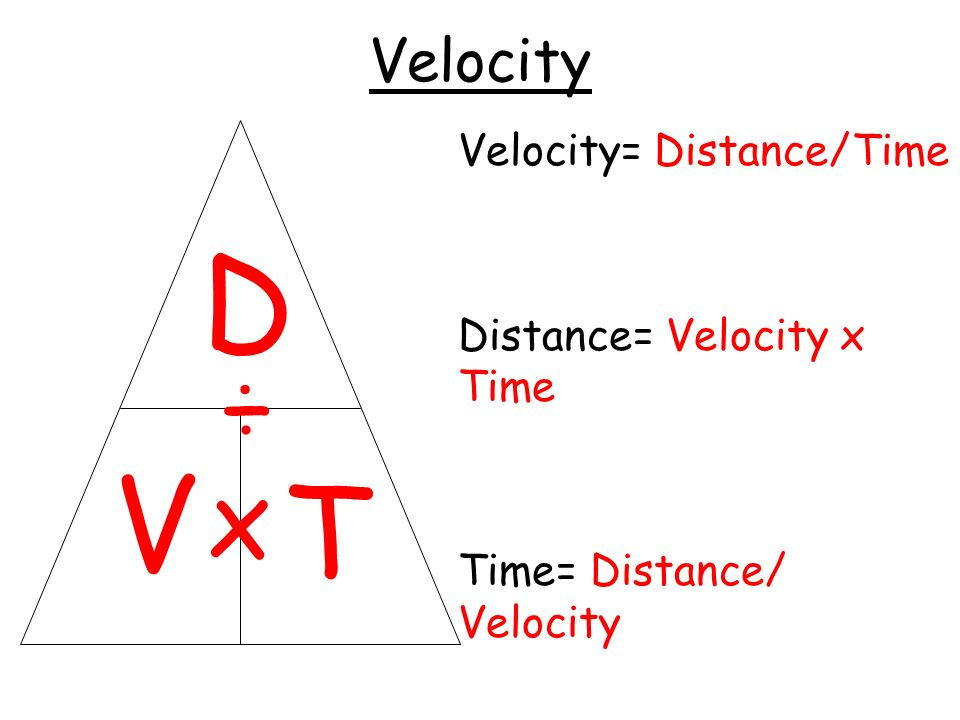
\includegraphics[scale=.3]{Velocity.jpeg}

\subsection{Boxing Workouts}
\newpage
\subsection{Nutrition in Relation To sports}
\subsection{Integration Of Ionic, Cordova, Angular}

\subsection{Tensorflow, Firebase}

\subsection{Android}

\subsection{Deploying on the App Store}

\subsection{Wearable Devices}

\subsection{Survey, Results}

\subsection{Future Improvements}




\subsection{Artificial Neural Network}
In the oxford dictionary it says, “artificial intelligence is an area of study concerned with making computers copy intelligent human behaviour \cite{knowles2006oxford}.” If you google the question that I just asked, you’ll get something like “the theory and development of computer systems able to perform tasks normally requiring human intelligence, such as visual perception, speech recognition, decision-making, and translation between languages.”

To really understand what Artificial intelligence (AI) is, we first must know what Intelligence is. When people talk about intelligence, they identify it with “the ability to solve hard problems.” Some people say it’s “Maybe it is too early
to define intelligence. It is obvious that, after decades of study, we still do not know very much about it. There are more questions than answers \cite{wang2007logic}.” This is where we stumble upon the idea of Artificial Intelligence.
\textbf{The birth of the idea}
\\
The birth of AI is bizarre from what normal people would think. AI wasn’t made along with computers it was sort of this fictional monster. The first AI possibly made was by Mary Shelly when she wrote Frankenstein in 1818 \cite{shelley2012frankenstein}.So technically the first ever AI was made long before we even thought of the idea. The main concept that comes into people’s minds is something man made that is designed to solve all our lives biggest questions. \cite{bostrom2014ethics}

For this project we have to learn how to build a neural database. To build the actual neural network we are using a program called Keras which comes with Anaconda, a powerful tool used with Python. We look at different approaches when it comes to training a system. For example, taking this project in hand, we need to train the system to recognize the different types of punches thrown. Before learning out neural networks we would need to know what a neuron is.\\
\textbf{Neuron}

\textit{"A specialized cell transmitting nerve impulses; a nerve cell."} \\ A neuron has an input($x$) and output($y$). The input normally has a weight to it and a bias($b$) with is usually This image below will show you how a neuron looks.
\\
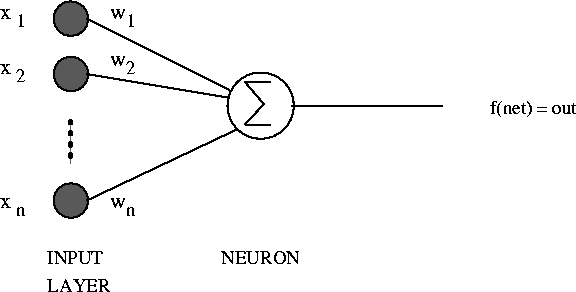
\includegraphics[scale=.4]{images/Neuron.png}
\\
Neural networks are a set of algorithms, modeled loosely after the human brain, that are designed to recognize patterns. Neural networks are being applied to many real-life problems today, including speech and image recognition, spam email filtering, finance, and medical diagnosis, to name a few.

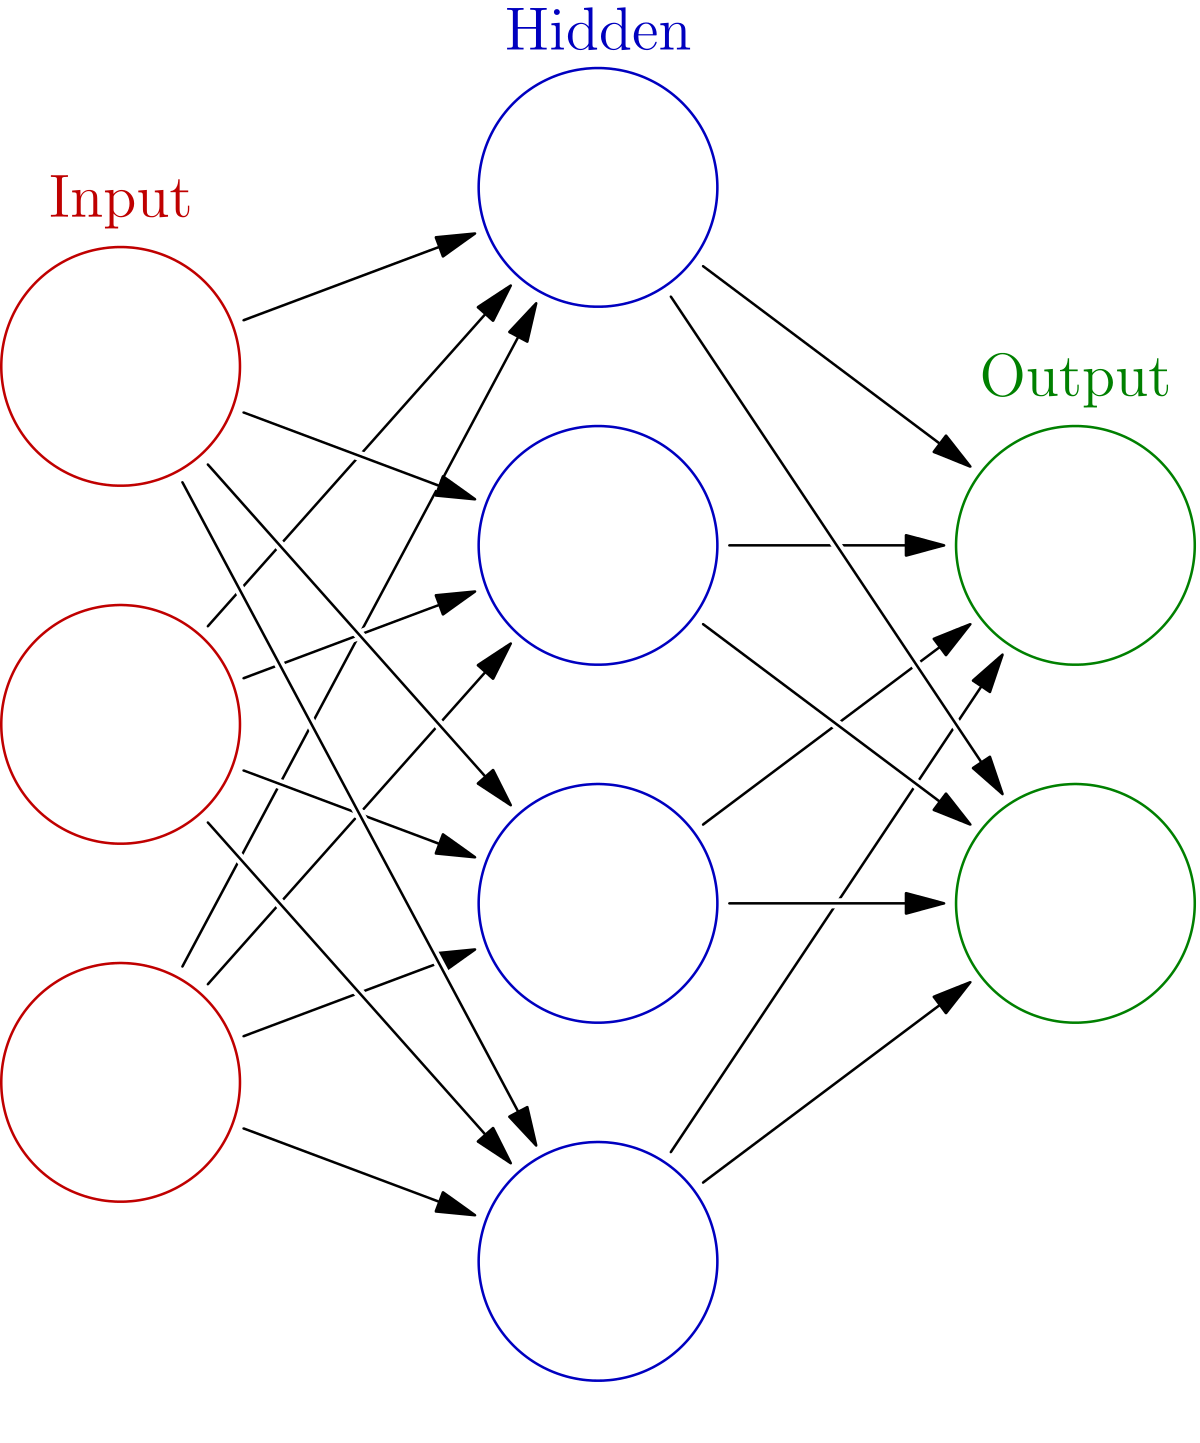
\includegraphics[scale=.19]{images/NeuralNetwork.png}
\\
\textbf{3 reasons to study neural computation:}\\
\textbf{1.} To understand how the brain actually works: it's very large and very complicated and made from things that die when you poke it, so we need to use computer simulations.\\
\textbf{2.} To grasp a neuron-inspired model of parallel computation and their adaptive connections: it is a very different style from sequential computation.\\
\textbf{3.} To solve practical problems by using novel learning algorithms inspired by the brain: learning algorithms can be very useful even if they are not how the brain actually works.
\\
With these tools, we can train the model to recognize the type of punches:\\
\textit{Jab\\hook\\Uppercut}

Using tensorflow with python to do this project. Tensorflow is a symbolic math library which can be used for machine learning. Keras is used to make the neural network. Numpy and pyplot is used to plot the data. Before making the data set for machine learning we'd need to learn of the core core concepts of making data-sets. This is how to shape your data and how to get it ready for training. To understand the layout of data-sets I used some examples online and decided to use the well know the iris data-set. This data-set collects data points from a hundred and fifty different samples of flower. It uses the petal length/width and the sepal length/width and sorts them into three types of iris.
\begin{verbatim}
from sklearn.datasets import load_iris

iris = load_iris()
iris

'data': array([[5.1, 3.5, 1.4, 0.2],
               [4.9, 3.0, 1.4, 0.2],
               [4.7, 3.2, 1.3, 0.2],
               [4.6, 3.1, 1.5, 0.2],
\end{verbatim}
I wanted to do something similar to this using the x,y,z axis on the device and the accelerometer and sorting them into the three types of punches the device would register. I've learnt that by training a neural network with these values and telling it the type of punch it is I can then build a neural network than can reference from new values what type of punch is thrown. The dataset that I'm going to make will contain four values and the type of punch it should be. The punch will be classified as 0, 1 or 2.

\subsection*{How is physics applied to boxing}
Physics occurs in punching because of energy. Person uses energy in order for a punch to be carried out. That is why, as well as energy we need momentum, work, power, and velocity. Before a boxer punches, he has potential energy which is stored energy. Once, the boxer begins to punch potential energy turns into kinetic energy.

Boxing is more than the brutal beating up of one another; it is a sport that applies many physics laws. If a fighter uses physics correctly, he will likely get the victory; but if he does not, he will probably lose.

As soon as a boxer starts to move his or her shoulders and arms and eventually the fists, his/her potential energy is being converted into kinetic energy.\\
\textbf{Kinetic energy is calculated by using the formula:}

$Kinetic Energy = (1/2)mv^2$

The fist has its maximum velocity when it hits something. The collision then causes the fist to slow down, eventually the fighter begins applying a force to retract his/her arm.\\
\textbf{This speed is calculated using:}

$Velocity = Distance / Time$
\\
What is Velocity? The speed of something in a given direction.

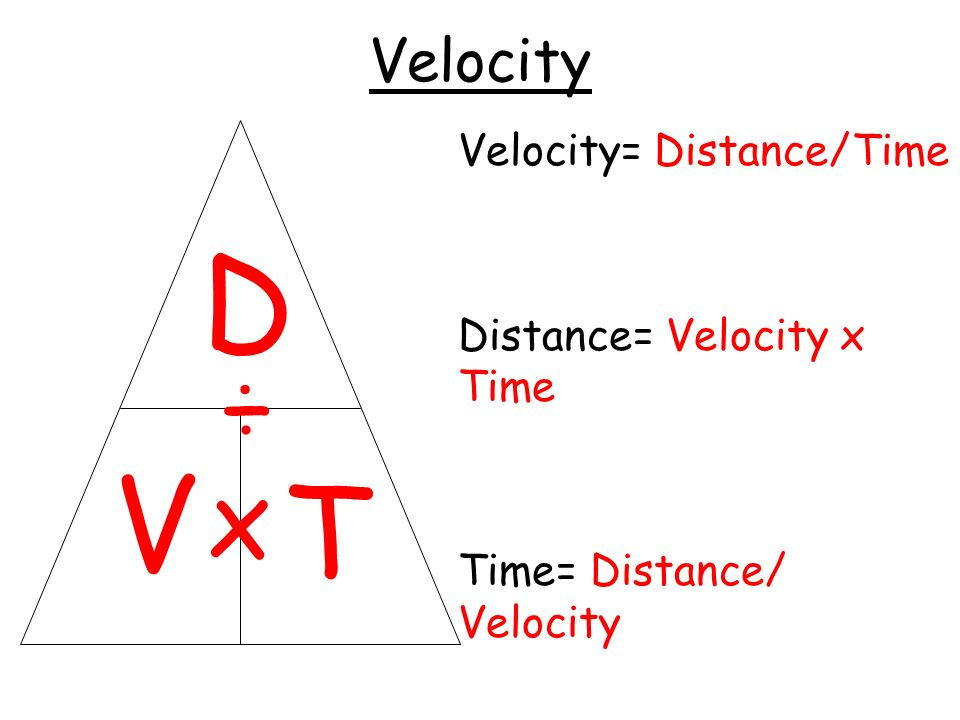
\includegraphics[scale=.3]{Velocity.jpeg}

\Chapter{Methodology}
\subsection{Work allocation}
We are allocating this project into three sections.
\textbf{First Step:}

Firstly we are going to start our research. We are going to deeply research in how this wearable device is going to work and what it takes to develop this new piece of technology. We need to understand what language is going to be used in constructing this. We need to know what sensors are required and how all data is going to be recorded.
\\
\textbf{Second Step:}

During the term our research is going to be a piece of document in how this wearable device can be achieved and possible drawing and animations of how it may work. But to back up our research, we need a physical piece that we can show and present. So we as a group decided to construct an application that is downloadable on mobile phone. This phone application is an alternative to the wearable device. The application is going to record the number of punches. The application is going to record and store data. For example is it going to store the number of punches under a certain amount of time.
\\
\textbf{Third Step:}

Whilst two members of the team are constructing the application. One person is going to specifically manage the database. They will have the responsibility to create the AWS account and link it up to the database. Overall, they are responsible for the whole database section of this project and to link it up to the application, that is works efficiently.

\subsection{Deployment}
We decided to android for developing our application. We choose android because the ease of use and developing. Android is one of many mobile operating systems based on the Linux kernel. Android was announced in Sept 2008 and has now become one of the most popular mobile operating system. Developing an app for android is simple using android studio and ionic. This is why we also choose ionic for our application. 

To deploy an app in the play store we'd need to;
\\
* Understand the Developer Program: \\https://play.google.com/about/developer-content-policy/

Following these guidelines we keep us in good standing with google play store and most importantly keep our users safe and protected. An example of this would be, our app should only request permissions that are only used for core features of the app while keeping clear of what personal data we use.
\\
* Test against the quality guidelines:\\ https://developer.android.com/docs/quality-guidelines

This will be tested with our test cases.
 
\Chapter{System Design}

\Chapter{Conclusion}

% references section
\bibliographystyle{plain}
\bibliography{refs} % 


\end{document}
